%\documentclass[aspectratio=169]{beamer}
\documentclass[8pt,aspectratio=169,xcolor={table,dvipsnames,usenames}]{beamer}
\usefonttheme[onlymath]{serif}
\usepackage[brazilian]{babel}
\usepackage{animate}


\mode<presentation>
{
  \usetheme{Madrid}      % or try Darmstadt, Madrid, Warsaw, ...
  \usecolortheme{dolphin} % or try albatross, beaver, crane, ...
  \usefonttheme{default}  % or try serif, structurebold, ...
  \setbeamertemplate{navigation symbols}{}
  \setbeamertemplate{caption}[numbered]
  \setbeamertemplate{headline}{}
}

\usepackage{mathtools}
%\usepackage{amsthm}
\usepackage{amsmath}
%\usepackage{nccmath}
\usepackage{amssymb}
%\usepackage{amsfonts}
\usepackage{physics}
%\usepackage{dsfont}
%\usepackage{mathrsfs}
%\usepackage{slashed}    % Feynman slash notation, requires LuaLaTeX
%\usepackage[compat=1.1.0]{tikz-feynman}   % Feynman diagrams

%\usepackage{titling}
\usepackage{indentfirst}
%\usepackage[titletoc,title]{appendix}
%\renewcommand\appendixname{Apêndice}

\usepackage{bm}
%\usepackage{xcolor}
%\usepackage[dvipsnames]{xcolor}
\usepackage{cancel}

%\usepackage{xurl}
\usepackage{hyperref}
\usepackage{cite}

\usepackage{float}
\usepackage{graphicx}
\usepackage{tikz}
\usepackage{caption}
\usepackage{subcaption}

%%%%%%%%%%%%%%%%%%%%%%%%%%%%%%%%%%%%%%%%%%%%%%%%%%%

\newcommand{\eps}{\epsilon}
\newcommand{\vphi}{\varphi}
\newcommand{\cte}{\text{cte}}

\newcommand{\N}{\mathbb{N}}
\newcommand{\Z}{\mathbb{Z}}
\newcommand{\Q}{\mathbb{Q}}
\newcommand{\R}{\vb{R}}
\newcommand{\C}{\mathbb{C}}
\renewcommand{\S}{\vb{S}}
%\renewcommand{\H}{\s{H}}

\renewcommand{\a}{\vb{a}}
\renewcommand{\b}{\vb{b}}
\renewcommand{\d}{\dagger}
\newcommand{\up}{\uparrow}
\newcommand{\down}{\downarrow}
\newcommand{\hc}{\text{h.c.}}

\newcommand{\0}{\vb{0}}
\newcommand{\1}{\mathds{1}}
\newcommand{\E}{\vb{E}}
\newcommand{\B}{\vb{B}}
\renewcommand{\v}{\vb{v}}
\renewcommand{\r}{\vb{r}}
\renewcommand{\k}{\vb{k}}
\newcommand{\p}{\vb{p}}
\newcommand{\q}{\vb{q}}
\newcommand{\F}{\vb{F}}
\newcommand{\A}{\vb{A}}
\newcommand{\J}{\vb{J}}

\newcommand{\s}{\sigma}
\newcommand{\nn}[2]{\left\langle #1 , #2 \right\rangle}
\newcommand{\cc}[1]{\overline{#1}}
\newcommand{\Eval}[3]{\eval{\left( #1 \right)}_{#2}^{#3}}

\newcommand{\unit}[1]{\; \mathrm{#1}}

\newcommand{\n}{\medskip}
\newcommand{\e}{\quad \mathrm{e} \quad}
\newcommand{\ou}{\quad \mathrm{ou} \quad}
\newcommand{\virg}{\, , \;}
\newcommand{\ptodo}{\forall \,}
\renewcommand{\implies}{\; \Rightarrow \;}
%\newcommand{\eqname}[1]{\tag*{#1}} % Tag equation with name


%%%%%%%%%%%%%%%%%%%%%%%%%%%%%%%%%%%%%%%%%%%%%%%%%%%%%%%%%

\title[Introdução ao Twisted Bilayer Graphene]{\LARGE{Introdução ao Twisted Bilayer Graphene}}
\author[Mateus Marques]{
\large{Mateus Marques
}}
\date{\today}

\begin{document}

\begin{frame}
  \titlepage
\end{frame}


\begin{frame}{Grafeno}

\begin{itemize}
\item O grafeno é derivado do grafite (do seu lápis)

\item Uma única camada de grafite e mantido estável num substrato (SiO$_2$, hBN etc.)

\item Cristal 2D de átomos de carbono numa rede hexagonal (favo de mel)

\item Pelas ligações covalentes C$-$C, é cerca de 200 vezes mais forte que o aço

\item Incrivelmente leve, flexível e quase completamente transparente

\item Conduz eletricidade melhor do que o cobre, dissipa calor de maneira extremamente eficiente
\end{itemize}

\begin{figure}[H]
\centering
\includegraphics[height=0.25\linewidth]{fig/graphene.png}
%\caption{Estrutura do grafeno. Figura retirada de \url{https://sitn.hms.harvard.edu/flash/2011/graphene-the-coolest-material-that-shouldnt-exist/}.}
\label{fig:graphene}
\end{figure}

\end{frame}

%%%%%%%%%%%%%%%%%%%%%%%%%%%%%%%%%%%%%%%%%%%%%%%%%%%%%%%%%%%%%%%%%%%%%%%%%%%%%%%%%%%%%%%%%%%%%%%%%

\begin{frame}{Padrão de moiré}

Empilhamos duas camadas de grafeno e giramos por um ângulo $\theta \implies$ padrão de Moiré.

\begin{figure}[H]
\centering
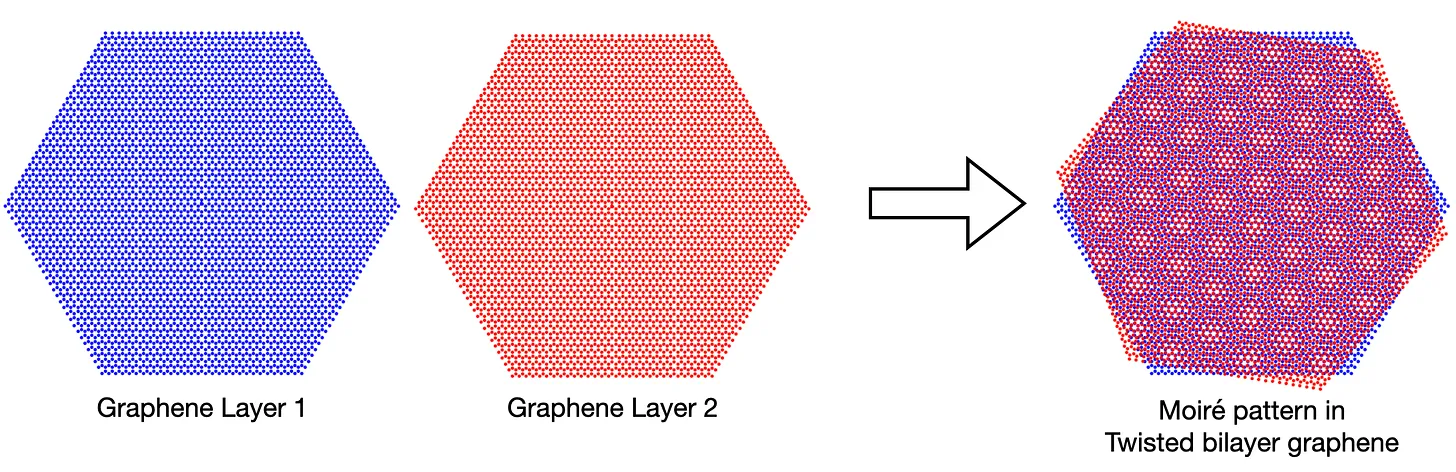
\includegraphics[height=0.30\linewidth]{fig/moire.png}
%\caption{Padrão de moiré. Retirada de \url{https://arpitarora22.substack.com/p/artful-probe-for-quantum-magic-in}.}
\label{fig:moire}
\end{figure}

Surge um novo cristal (ou não), com constante de rede maior $L(\theta)$
$$
L(\theta) = \abs{r(\theta)} \, L_m(\theta), \quad L_m(\theta) = \frac{a}{2 \sin(\theta/2)}, \quad r(\theta) \in \Z^*.
$$

Não é para todo ângulo $\theta$ que a nova estrutura é \textit{comensurável}.

\end{frame}

%%%%%%%%%%%%%%%%%%%%%%%%%%%%%%%%%%%%%%%%%%%%%%%%%%%%%%%%%%%%%%%%%%%%%%%%%%%%%%%%%%%%%%%%%%%%%%%%%

\begin{frame}{Scanning tunneling microscope (STM)}

\begin{figure}[H]
\centering
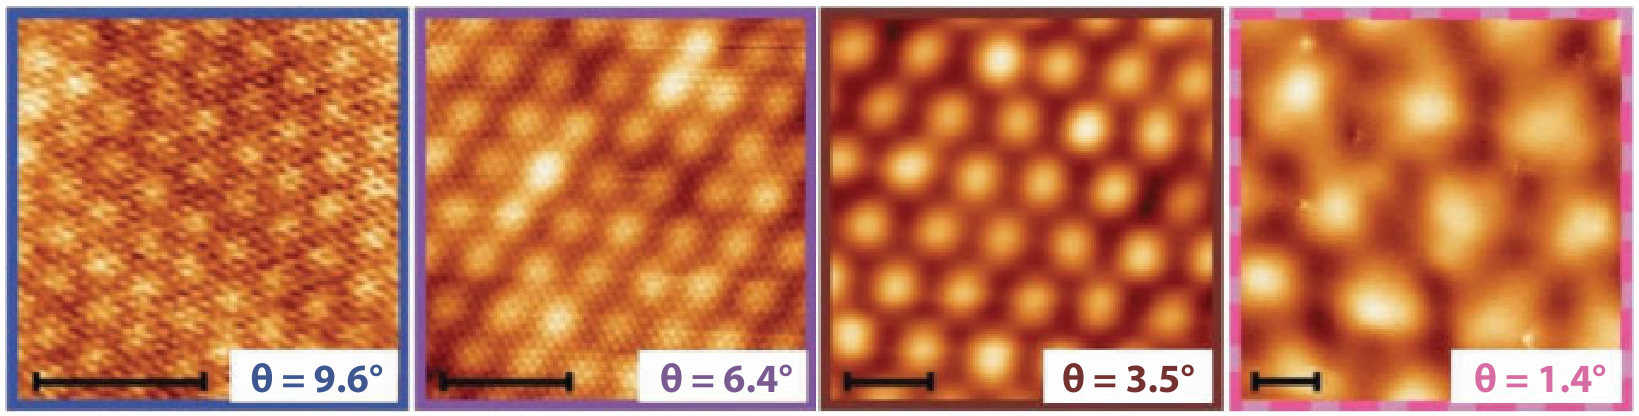
\includegraphics[width=\linewidth]{fig/stm.png}
\caption{Padrão de moiré observado em STM. As barras de escala são de 5 nm. Retirada de \cite{handbook2019}.}
\label{fig:stm}
\end{figure}

Observe que a constante de rede tem ordem de \textbf{nanômetros} para $\theta \lesssim 5^\circ$, ou seja, a célula unitária do novo sistema é \textbf{muito grande}.

\n

Para $\theta=1.1^\circ$ temos em torno de 11000 átomos na célula unitária \cite{rennella}.

\end{frame}

%%%%%%%%%%%%%%%%%%%%%%%%%%%%%%%%%%%%%%%%%%%%%%%%%%%%%%%%%%%%%%%%%%%%%%%%%%%%%%%%%%%%%%%%%%%%%%%%%

\begin{frame}{Magic-Angle Twisted Bilayer Graphene (MATBG)}

Ao se aproximar do ângulo ``mágico'' $\theta \approx 1.05^\circ$, várias propriedades interessantes são amplificadas.
\begin{itemize}
\item Transição metal-isolante de Mott \cite{cao2018-insulator}.
\item Supercondutividade não-convencional tunável \cite{cao2018-superconductivity}, com $T_c = 1.7 \unit{K}$.
\item Bandas planas com topologia não-trivial \cite{rennella}.
\end{itemize}

\begin{figure}[H]
\centering
\begin{subfigure}{.58\textwidth}
  \centering
  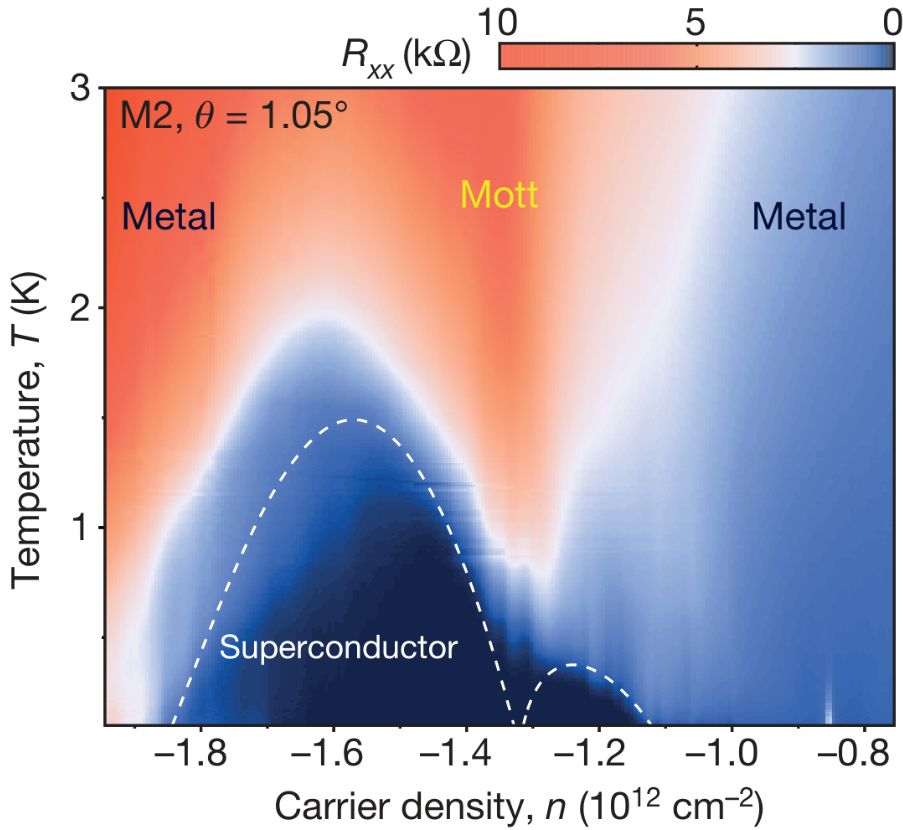
\includegraphics[height=13em]{fig/matbg-superconductivity.png}
  \label{fig:matbg-superconductivity}
\end{subfigure}%
\quad
\begin{subfigure}{.38\textwidth}
  \centering
  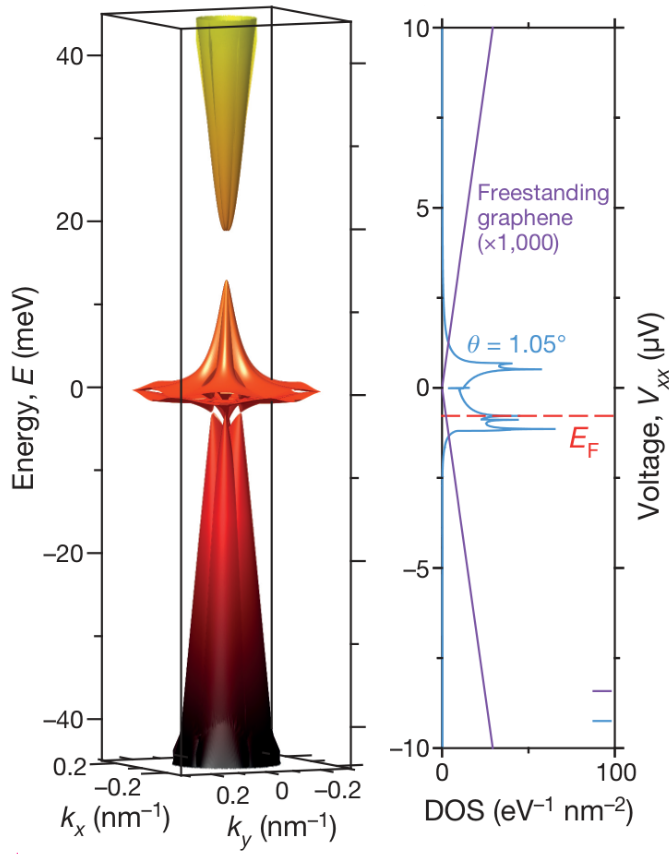
\includegraphics[height=13em]{fig/matbg-bands.png}
  \label{fig:matbg-bands}
\end{subfigure}
\caption{Diagramas de fase e de bandas do MATBG, $\theta = 1.05^\circ$. Figura retirada de \cite{cao2018-superconductivity}.}
\label{fig:matbg-exp}
\end{figure}

\end{frame}


%%%%%%%%%%%%%%%%%%%%%%%%%%%%%%%%%%%%%%%%%%%%%%%%%%%%%%%%%%%%%%%%%%%%%%%%%%%%%%%%%%%%%%%%%%%%%%%%%

\begin{frame}

\begin{center}
\huge Como abordar esse sistema teoricamente?
\end{center}

\n\n\n\n

\begin{itemize}
\item É um sistema bastante recente, com muito interesse, muito debate e pouco consenso.
\item Na literatura existem $10^{538}$ modelos diferentes.
\item Uma das abordagens que é uma \textbf{base} para muitas outras é o modelo contínuo, que incorpora as principais ``boas'' simetrias do TBG.
\end{itemize}

\end{frame}

%%%%%%%%%%%%%%%%%%%%%%%%%%%%%%%%%%%%%%%%%%%%%%%%%%%%%%%%%%%%%%%%%%%%%%%%%%%%%%%%%%%%%%%%%%%%%%%%%

\begin{frame}{Tight-binding no Grafeno}

\begin{figure}[H]
\centering
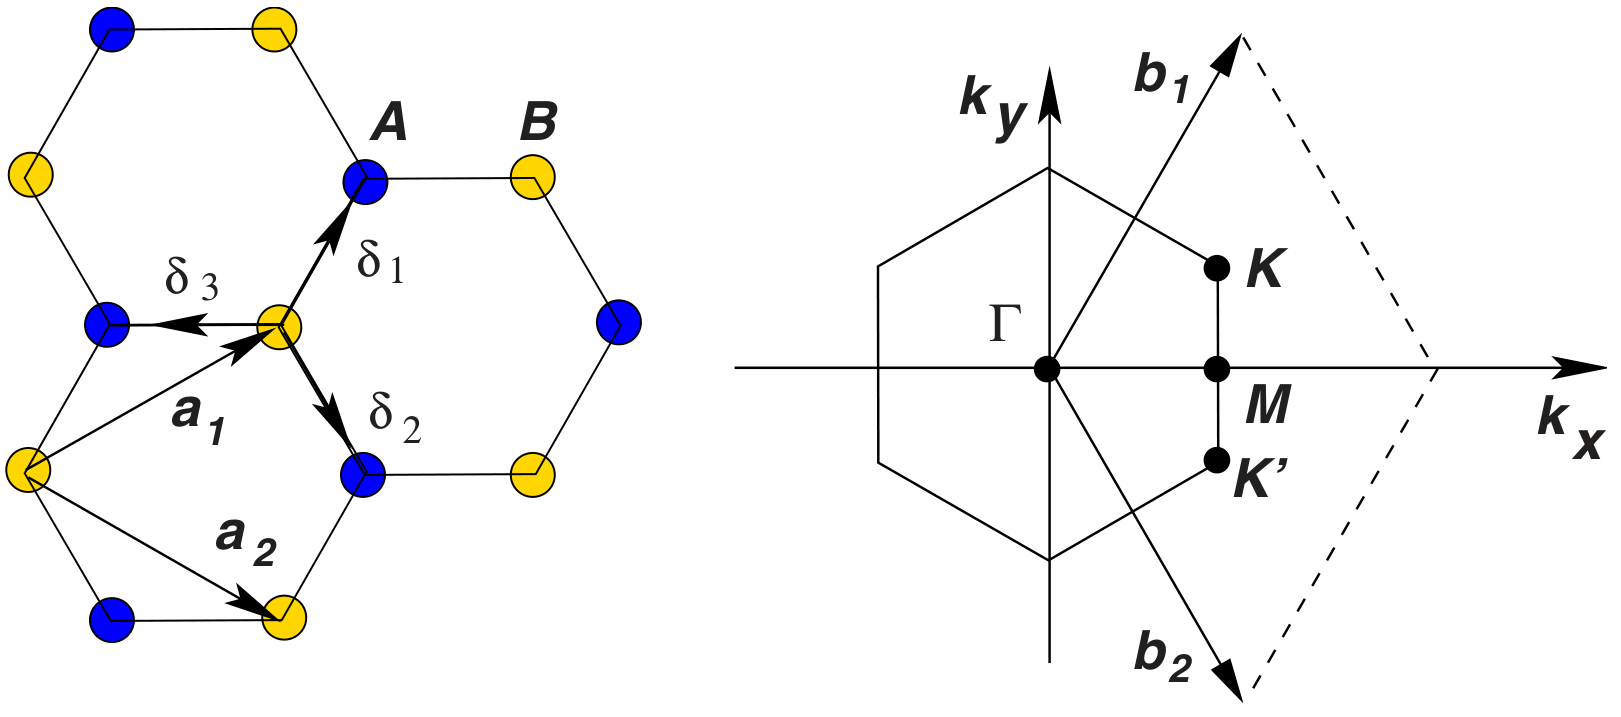
\includegraphics[width=0.5\linewidth]{fig/monolayer.png}
\caption{Rede direta e zona de Brillouin do grafeno usual. Figura retirada de \cite{castroneto}.}
\label{fig:monolayer}
\end{figure}

No grafeno comum geralmente é aplicado o método de tight-binding, onde escrevemos a hamiltoniana
$$
H = -t \sum_{\R} c^\d_B(\R) \qty(c_A(\R) + c_A(\R-\a_1) + c_A(\R-\a_2)) + \hc,
$$
que leva em conta os hoppings entre primeiros vizinhos dos sítios $A$ e $B$ do grafeno.

\end{frame}

%%%%%%%%%%%%%%%%%%%%%%%%%%%%%%%%%%%%%%%%%%%%%%%%%%%%%%%%%%%%%%%%%%%%%%%%%%%%%%%%%%%%%%%%%%%%%%%%%

\begin{frame}{Relação de dispersão no Grafeno}

Ao reescrever a hamiltoniana no espaço de momento, conseguimos diagonalizá-la
$$
H =
\begin{pmatrix}
0 & -t f(\k) \\
-t f^*(\k) & 0
\end{pmatrix}, \quad f(\k) = \sum_{\nu} e^{i \k \vdot \bm{\delta}_\nu},
$$
obtendo a relação de dispersão $E(\k) = \pm t \abs{f(\k)}$.

\begin{figure}[H]
\centering
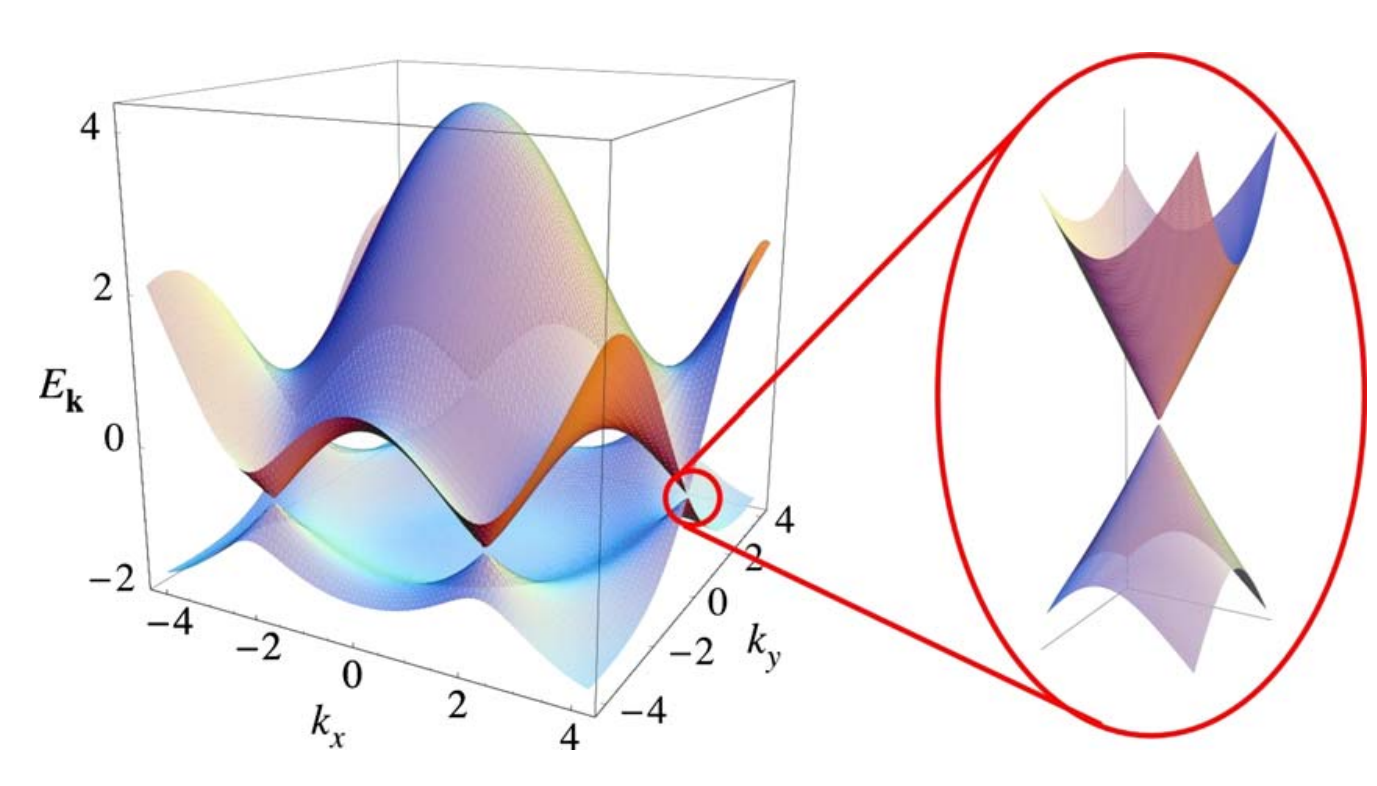
\includegraphics[height=0.3\linewidth]{fig/dirac.png}
\caption{Relação de dispersão do grafeno e cones de Dirac. Figura retirada de \cite{castroneto}.}
\label{fig:dirac}
\end{figure}

\end{frame}


%%%%%%%%%%%%%%%%%%%%%%%%%%%%%%%%%%%%%%%%%%%%%%%%%%%%%%%%%%%%%%%%%%%%%%%%%%%%%%%%%%%%%%%%%%%%%%%%%

\begin{frame}{Regime de baixas energias}

No limite de baixas energias, somente as regiões próximas dos pontos de Dirac $\K$ e $\K'$ importam.

\n

Em torno desses pontos, a relação de dispersão $E(\k)$ assume a forma de cone (dispersão relativística)
$$
E(\K+\q) \approx \pm \hbar v_F \abs{\q}.
$$

\n

Pensando no TBG, caso rodemos essa camada de grafeno por um ângulo $\theta$, sua hamiltoniana de baixas energias será
$$
H^\theta(\q) = \hbar v_F \abs{\q}
\begin{pmatrix}
0 & e^{-i(\theta_\q - \theta)} \\
e^{i(\theta_\q - \theta)} & 0
\end{pmatrix}.
$$

\n

Para modelar o TBG, utilizaremos a hamiltoniana acima para cada uma das duas camadas. Porém, ainda temos que levar em conta a hibridização entre elas.

\end{frame}

%%%%%%%%%%%%%%%%%%%%%%%%%%%%%%%%%%%%%%%%%%%%%%%%%%%%%%%%%%%%%%%%%%%%%%%%%%%%%%%%%%%%%%%%%%%%%%%%%

\begin{frame}{Modelo contínuo}

\begin{itemize}
\item Hamiltoniana de tight-binding para a hibridização entre as duas camadas.
\item Interações do TBG são de longo alcance, devido à interferência do padrão de Moiré.
\item Ao invés de tight-binding no espaço direto, consideramos hoppings entre primeiros vizinhos no \textbf{espaço de momento}.
\end{itemize}

\begin{figure}[H]
\centering
\begin{subfigure}{.48\textwidth}
  \centering
  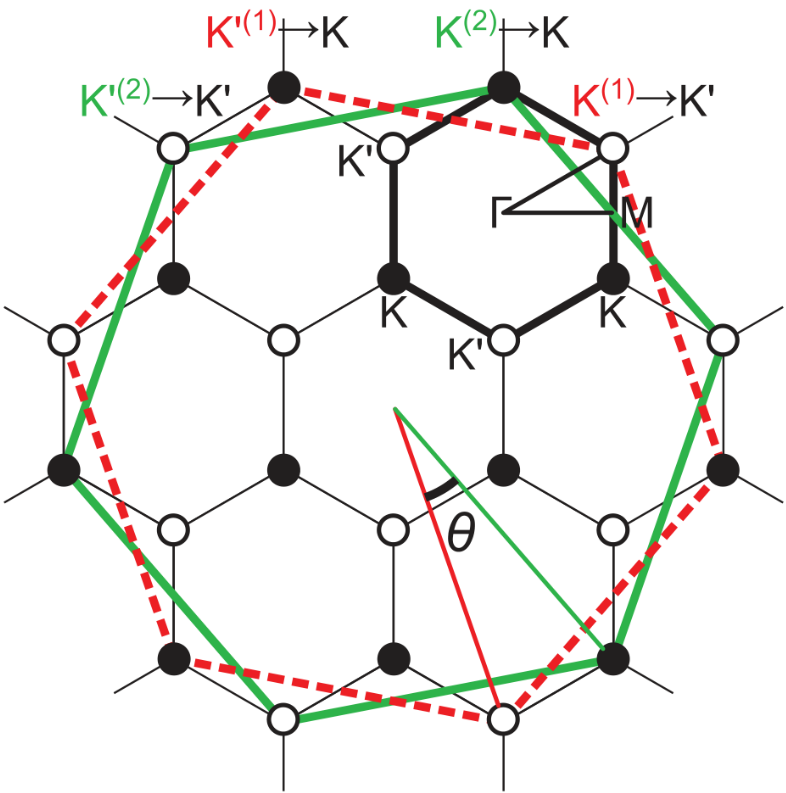
\includegraphics[height=18em]{fig/minibz.png}
  \label{fig:minibz}
\end{subfigure}%
\quad
\begin{subfigure}{.48\textwidth}
  \centering
  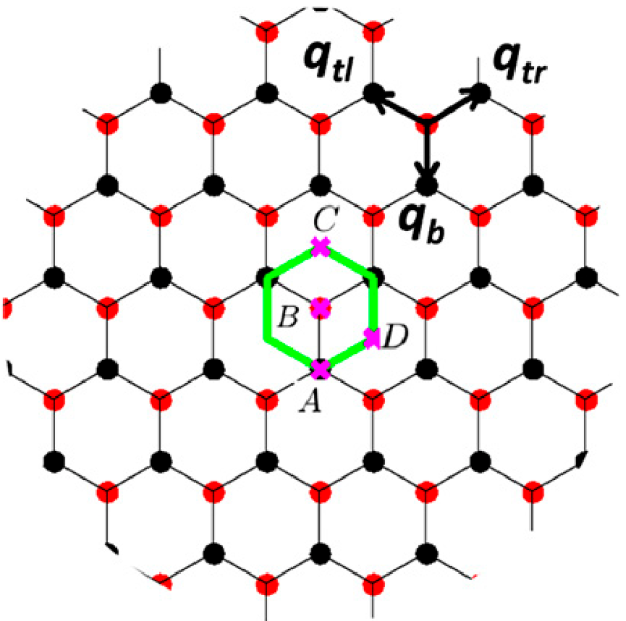
\includegraphics[height=18em]{fig/tightbinding-q.png}
  \label{fig:tightbinding-q}
\end{subfigure}
\caption{Mini zona de Brillouin e hoppings no espaço de momento do TBG. Figuras retiradas de \cite{koshino} e \cite{macdonald}.}
\label{fig:tbg-bz}
\end{figure}


\end{frame}

%%%%%%%%%%%%%%%%%%%%%%%%%%%%%%%%%%%%%%%%%%%%%%%%%%%%%%%%%%%%%%%%%%%%%%%%%%%%%%%%%%%%%%%%%%%%%%%%%

\begin{frame}{Modelo contínuo}

O modelo contínuo consegue explicar o surgimento de bandas planas na dispersão do TBG.

\begin{center}
\animategraphics[loop,height=20em,controls]{6}{fig/bands-}{0}{109}
\end{center}

\end{frame}


%%%%%%%%%%%%%%%%%%%%%%%%%%%%%%%%%%%%%%%%%%%%%%%%%%%%%%%%%%%%%%%%%%%%%%%%%%%%%%%%%%%%%%%%%%%%%%%%%

\begin{frame}{Discussão de simetrias do TBG}

Dependendo do ângulo $\theta$ e escolha do centro de rotação, a estrutura do TBG pode ter diferentes grupos de simetrias exatas. Para $\theta = 3.89^\circ$, a Figura \ref{fig:AA_AB} mostra um exemplo disso onde uma estrutura tem simetria $D_3$ e outra $D_6$.

\begin{figure}[H]
\centering
\begin{subfigure}{.48\textwidth}
  \centering
  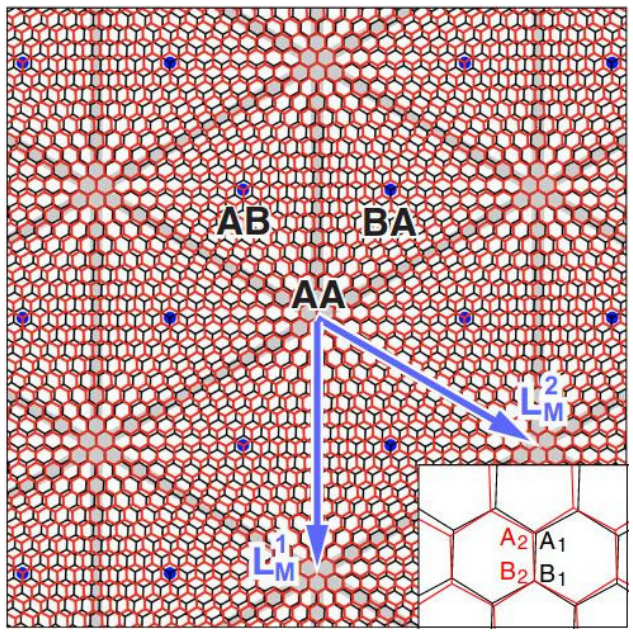
\includegraphics[height=18em]{fig/AA_AB-D3.png}
  \label{fig:AA_AB-D3}
\end{subfigure}%
\quad
\begin{subfigure}{.48\textwidth}
  \centering
  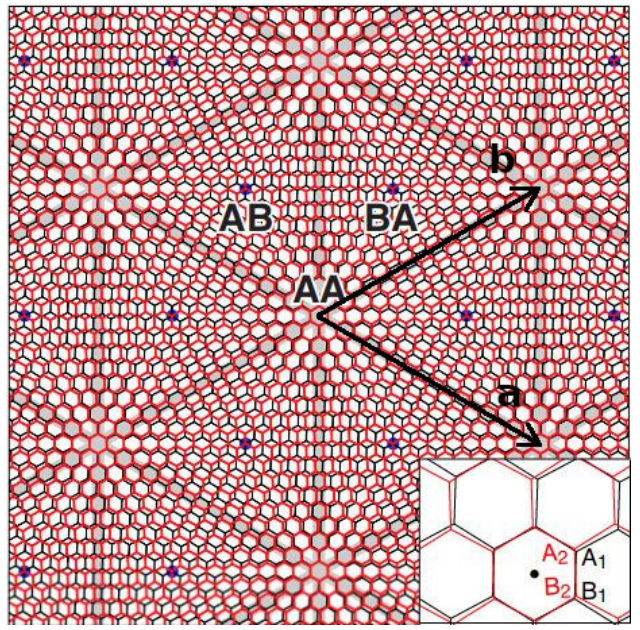
\includegraphics[height=18em]{fig/AA_AB-D6.png}
  \label{fig:AA_AB-D6}
\end{subfigure}
\caption{Estrutura atômica do TBG para $\theta = 3.89^\circ$ com simetrias $D_3$ (direita) e $D_6$ (esquerda). Figuras retiradas de \cite{rennella}.}
\label{fig:AA_AB}
\end{figure}
\vspace{-1em}
Em experimentos reais, observa-se a robustez de simetrias emergentes de translação, de vale $U_v(1)$, de reversão temporal com rotação $C_2 \mathcal{T}$, e de grupo pontual $D_6$. Essas simetrias não são exatas para qualquer ângulo $\theta$, mas pelas escalas de energia observada em experimentos, é como se o sistema incorporasse todas essas \textbf{boas simetrias} \cite{zou}.

\end{frame}

%%%%%%%%%%%%%%%%%%%%%%%%%%%%%%%%%%%%%%%%%%%%%%%%%%%%%%%%%%%%%%%%%%%%%%%%%%%%%%%%

\begin{frame}{Referências}

\scriptsize

\begin{thebibliography}{10}

\bibitem{rennella}
\alert{Rennella Roberto}
\newblock{Symmetry analysis of twisted bilayer graphene (TBG)}
\newblock{Master Thesis -- Università Degli Studi di Napoli Federico II, 2019.}

\bibitem{handbook2019}
\alert{G. Catarina, B. Amorim, E. V. Castro, J. M. V. P. Lopes, N. Peres}
\newblock{Twisted Bilayer Graphene: Low-Energy Physics, Electronic and Optical Properties}
\newblock{Handbook of Graphene -- Chapter 6, John Wiley \& Sons, Ltd, 2019.}

\bibitem{cao2018-insulator}
\alert{Y. Cao, V. Fatemi, S. Fang, et al}
\newblock{Correlated insulator behaviour at half-filling in magic-angle graphene superlattices}
\newblock{\textit{Nature}, vol. 556, p. 8084, Mar 2018.}

\bibitem{cao2018-superconductivity}
\alert{Y. Cao, V. Fatemi, S. Fang, et al}
\newblock{Unconventional superconductivity in magic-angle graphene superlattices}
\newblock{\textit{Nature}, vol. 556, pp. 43-50, Apr 2018.}

\bibitem{castroneto}
\alert{A. H. Castro Neto, F. Guinea, N. Peres, K. Novoselov, A. Geim}
\newblock{The electronic properties of graphene}
\newblock{\textit{Rev. Mod. Phys.}, vol. 81, pp. 109-162, Jan 2009.}

\bibitem{zou}
\alert{L. Zou, H. C. Po, A. Vishwanath, T. Senthil}
\newblock{Band structure of twisted bilayer graphene: Emergent symmetries, commensurate approximants, and Wannier obstructions}
\newblock{\textit{Physical Review B}, vol. 8, no. 85435, 2018.}

\bibitem{koshino}
\alert{P. Moon, M. Koshino}
\newblock{Energy spectrum and quantum hall effect in twisted bilayer graphene}
\newblock{\textit{Phys. Rev. B}, vol. 85, p. 195458, May 2012}

\bibitem{macdonald}
\alert{R. Bistritzer, A. H. MacDonald}
\newblock{Moiré bands in twisted double-layer graphene}
\newblock{\textit{Proceedings of the National Academy of Sciences}, vol. 108, no. 30, pp. 12233–12237, 2011}

\end{thebibliography}


\end{frame}

\end{document}
